\NeedsTeXFormat{LaTeX2e}[1995/12/01]
\documentclass[10pt]{bmc_article}


% Load packages
%\usepackage{hyperref}
\usepackage{cite} % Make references as [1-4], not [1,2,3,4]
\usepackage{url} % Formatting web addresses
\usepackage{ifthen} % Conditional
\usepackage{multicol} %Columns
\usepackage{xspace}
\usepackage[utf8]{inputenc} %unicode support
%\usepackage[applemac]{inputenc} %applemac support if unicode package fails
%\usepackage[latin1]{inputenc} %UNIX support if unicode package fails
\urlstyle{rm}
\usepackage[OT1]{fontenc} 

\usepackage{rotating}
\usepackage{colortbl}
\usepackage{color}
\usepackage{comment}

\usepackage{subfigure}

\newcommand {\pg}[1]{\textcolor{blue}{#1}}
\newcommand {\ppg}[1]{\textcolor{blue}{#1}}
\newcommand {\new}[1]{\textcolor{green}{#1}}

\newcommand{\minitab}[2][l]{\begin{tabular}{#1}#2\end{tabular}}


%\newcommand{} {\mbox{}\xspace}

\def\squeezetable{\def\tabular@font{\tiny}}%

% Change useable area of a page to be slightly larger
\setlength{\topmargin}{0.0cm}
\setlength{\textheight}{21.5cm}
\setlength{\oddsidemargin}{0cm}
\setlength{\textwidth}{16.5cm}
\setlength{\columnsep}{0.6cm}

\newboolean{publ}

%Settings: comment\uncomment bmcformat definition to get format required

%Review style settings
\newenvironment{bmcformat}{\begin{raggedright}\baselineskip20pt\sloppy\setboolean{publ}{false}}{\end{raggedright}\baselineskip20pt\sloppy}

%Publication style settings
%\newenvironment{bmcformat}{\fussy\setboolean{publ}{true}}{\fussy}


% Begin ...
\begin{document}
\begin{bmcformat}

\title{Supplementary material for: non-coding RNAs of bird genomes}

\author{
Paul P. Gardner\correspondingauthor$^{1,2}$
\email{Paul P. Gardner\correspondingauthor - paul.gardner@canterbury.ac.nz},
Jana Hertel$^5$
\email{Jana Hertel\correspondingauthor - jana@bioinf.uni-leipzig.de},
Sarah W. Burge$^3$
\email{sb30@sanger.ac.uk},
Maria Ninova$^4$
\email{Maria.Ninova@postgrad.manchester.ac.uk},
Stephanie Kehr$^5$
\email{steffi@bierdepot.bioinf.uni-leipzig.de},
Mario Fasold$^5$
\email{mario@bierdepot.bioinf.uni-leipzig.de},
Tammy E. Steeves$^1$
\email{tammy.steeves@canterbury.ac.nz},
Sam Griffiths-Jones$^4$
\email{sam.griffiths-jones@manchester.ac.uk}
and
Peter Stadler\correspondingauthor$^5$
\email{Peter Stadler\correspondingauthor - studla@bioinf.uni-leipzig.de}
}
\address{
\iid(1) School of Biological Sciences, University of Canterbury, Private Bag 4800, Christchurch, New Zealand.
\iid(2) Biomolecular Interaction Centre, University of Canterbury, Private Bag 4800, Christchurch, New Zealand.
\iid(3) European Molecular Biology Laboratory, European Bioinformatics Institute, Hinxton, Cambridge, CB10 1SD, UK.
\iid(4) Faculty of Life Sciences, University of Manchester, Manchester, United Kingdom.
\iid(5) Bioinformatics Group, Department of Computer Science; and Interdisciplinary Center for Bioinformatics, University of Leipzig, H{\"a}rtelstrasse 16-18, D-04107 Leipzig, Germany
}

\maketitle

\begin{abstract}
...
\end{abstract}

%% Non-coding RNAs in bird genomes

%% Paul P. Gardner1,2, Sarah W. Burge3, Jana Hertel5, Maria Ninova4, Stephanie Kehr5, Anne Nitsche5, Mario Fasold5, Tammy E. Steeves1, Sam Griffiths-Jones4, Peter Stadler5

%% 1 School of Biological Sciences, University of Canterbury, Private Bag 4800, Christchurch, New Zealand. 2 Biomolecular Interaction Centre, University of Canterbury, Private Bag 4800, Christchurch, New Zealand. 3 European Molecular Biology Laboratory, European Bioinformatics Institute, Hinxton, Cambridge, CB10 1SD, UK. 4Faculty of Life Sciences, University of Manchester, Manchester, United Kingdom. 5 Bioinformatics Group, Department of Computer Science; and Interdisciplinary Center for Bioinformatics, University of Leipzig, Hartelstrasse 16-18, D-04107 Leipzig, Germany
 
%% Talking points:
%% 1. Although the majority of classical eukaryotic ncRNAs are conserved in birds, several notable classical ncRNAs are not. Homology searches in associated genes indicate these apparent "losses" are most likely due to divergence.
%% 2. Of the 59 snoRNA conserved between humans and yeast, we find 45 are conserved in birds. Homology searches in associated genes for the remaining non-conserved snoRNAs indicate these apparent losses are indeed due to multiple losses in several bird lineages.
%% 3. We find that 3 families of broadly conserved vertebrate microRNA families are lost in the avian lineage. We also annotate a number of bird-specific microRNAs.
%% 4. Several well-characterised lncRNA families of known function are conserved between mammals and birds.
%% 5. We discuss the conservation of HOX associated lncRNAs and several lncRNAs that have been implicated in processes associated with cancer.
 
%% %% Draft Abstract
%% We present the results of a large-scale bioinformatic annotation of non-coding RNAs in 48 avian genomes. We use probabilistic models of hand-curated families from the Rfam database to infer conserved RNA families within each avian genome. We supplement these annotations with predictions from the tRNA annotation tool, tRNAscan-SE, microRNAs from miRBase and selected sequences from analyses of the chicken transcriptome. Although we show extensive conservation of classical ncRNAs (e.g., tRNAs and rRNAs) and more recently discovered ncRNAs (e.g., snoRNAs and miRNAs) in birds, we also demonstrate apparent ``losses'' in several RNA families. These include the divergence of some classical ncRNAs and the genuine loss of several snoRNAs and microRNAs. In contrast, we show a signicant number of lncRNAs are surprisingly well conserved between birds and mammals including several intriguing cases where the reported mammalian lncRNA function is not conserved in birds. These combined results illustrate the utility of applying homology based methods for annotating vertebrate genomes and illustrate many complex evolutionary patterns within the avian ncRNA cohort.

%% LNCRNA:


\ifthenelse{\boolean{publ}}{\begin{multicols}{2}}{}

\section*{Supplementary introduction}
...

\section*{Supplementary results}
In the following we explore ...


\section*{Supplementary methods}
...



{\ifthenelse{\boolean{publ}}{\footnotesize}{\small}
\bibliographystyle{bmc_article} % Style BST file
 \bibliography{bird} } % Bibliography file (usually '*.bib' )

%%%%%%%%%%%

\clearpage
\newpage

\begin{figure}[ht]
  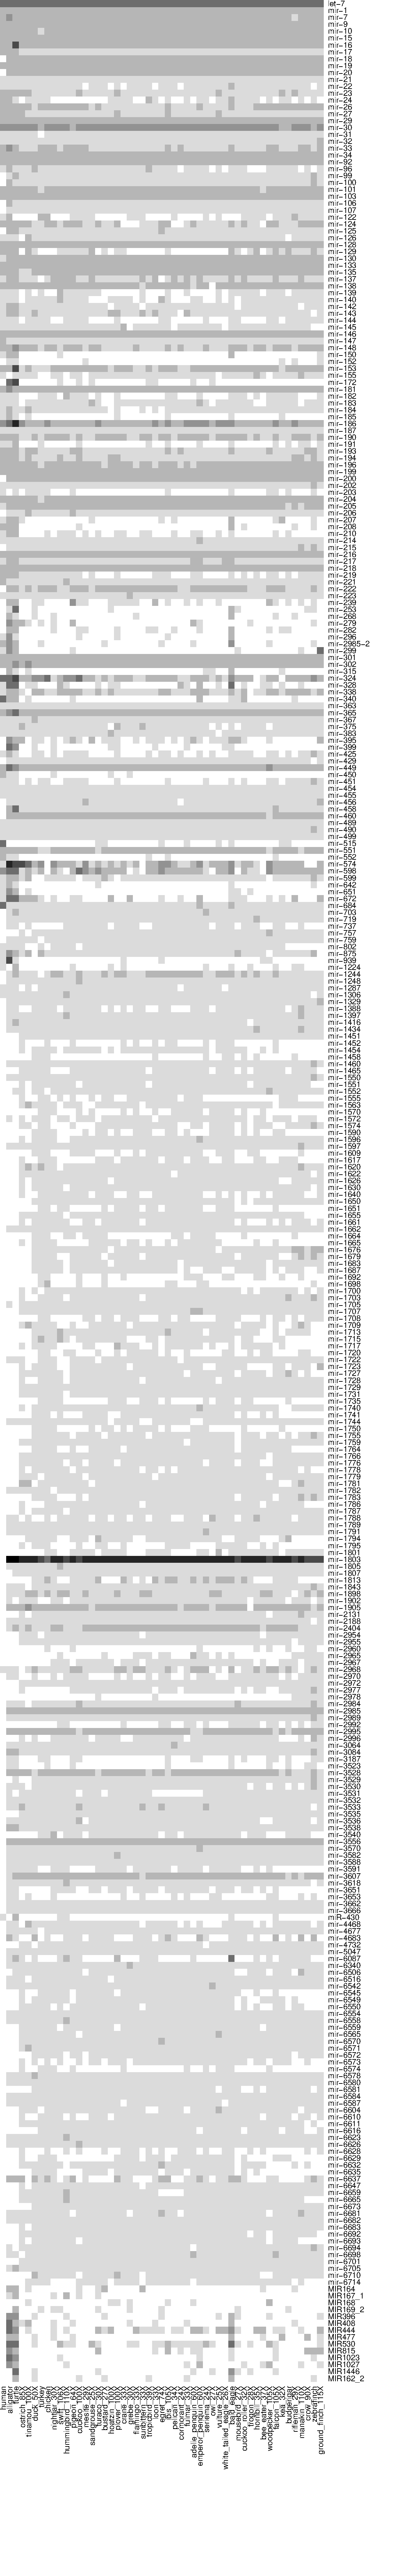
\includegraphics[height=0.95\textheight]{figures/miRNA.pdf}
  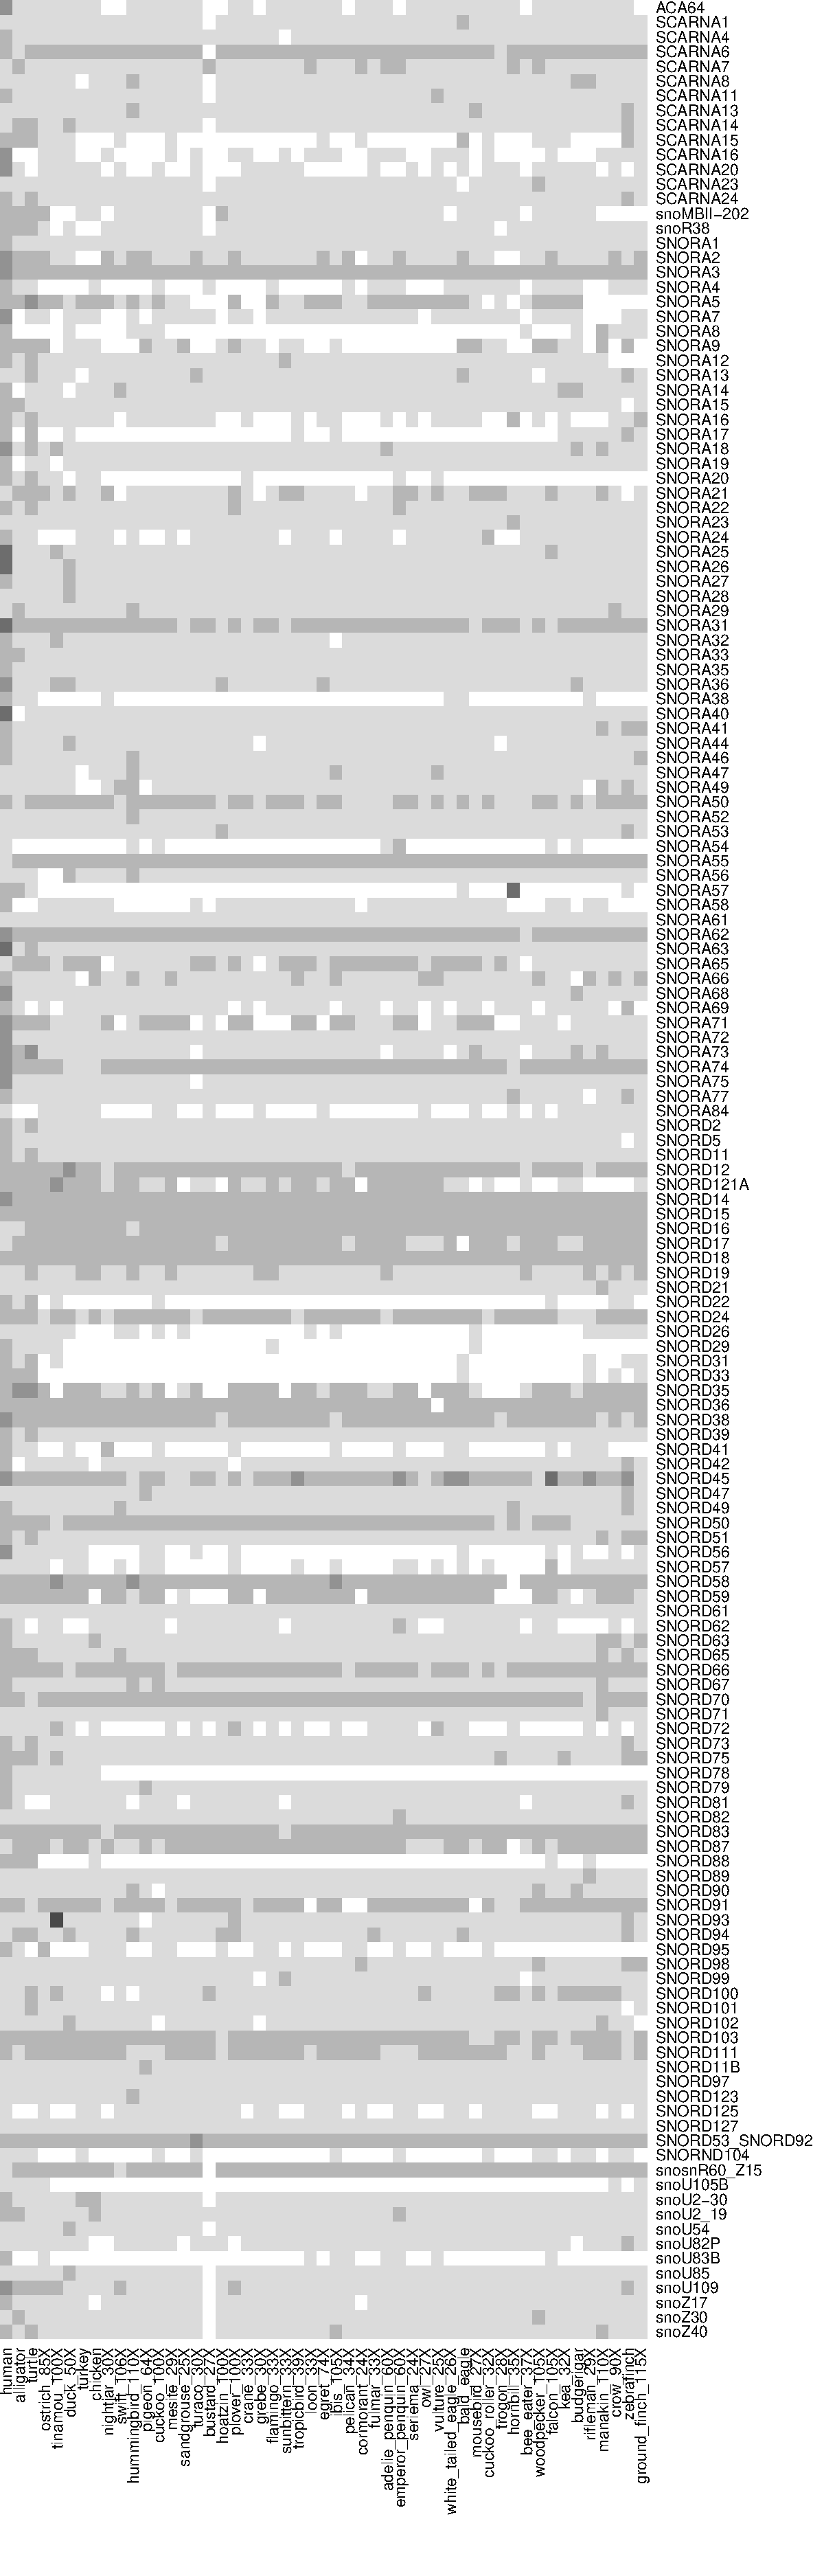
\includegraphics[height=0.95\textheight]{figures/snoRNA.pdf}
  \caption[]{Heatmaps showing the prescence/abscence and approximate
    copy number of {\bf miRNA} families on the right and {\bf snoRNA} families on
    the left.}\label{fig:3}
\end{figure}

\begin{figure}[ht]
  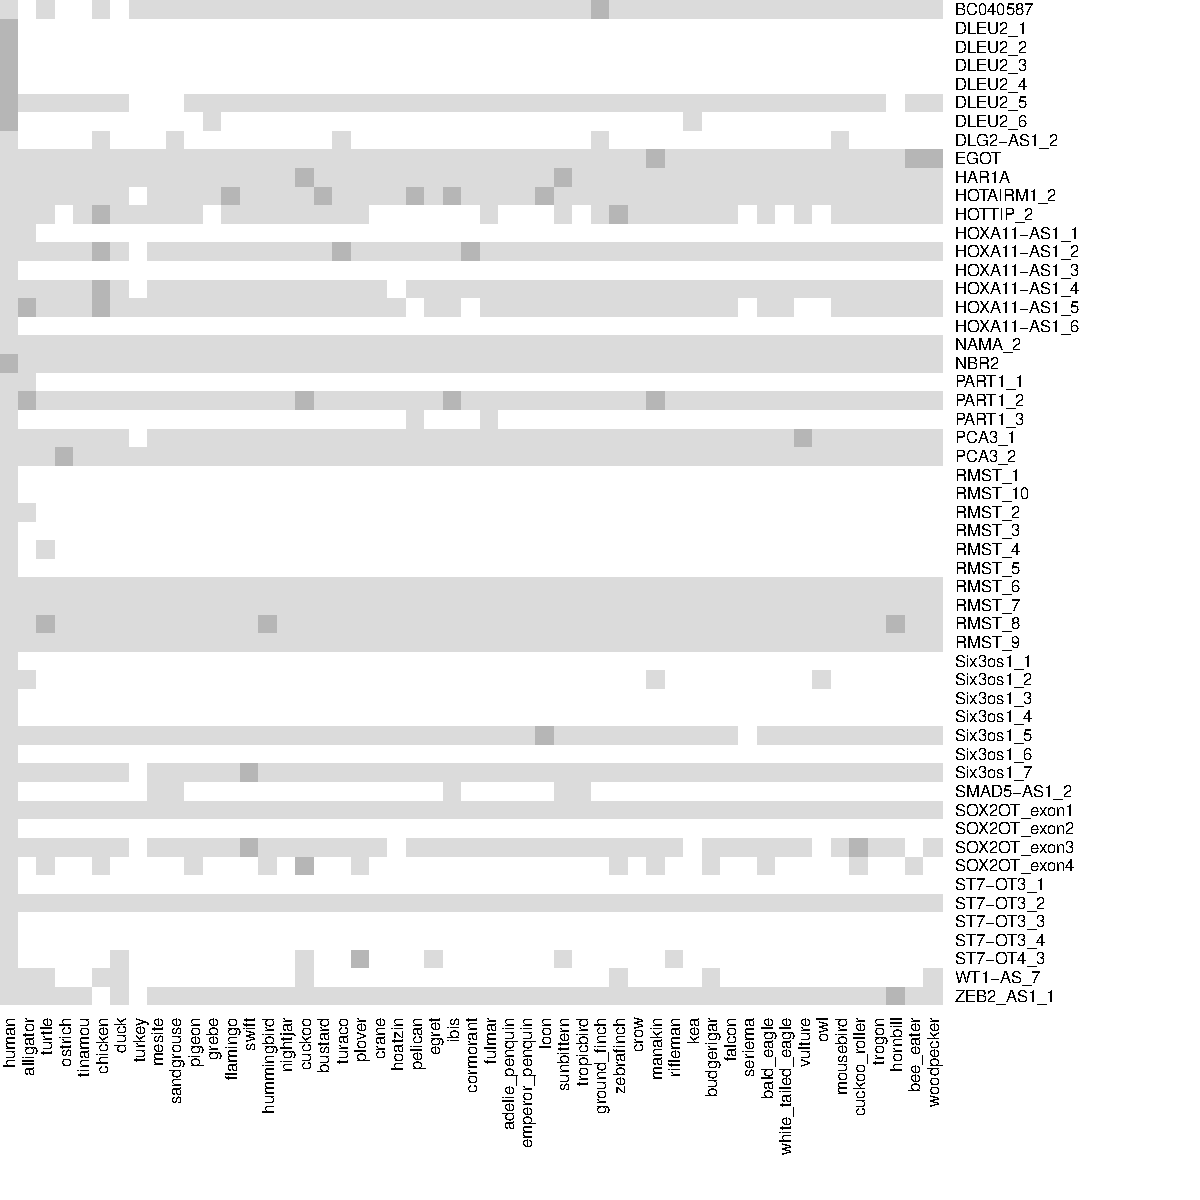
\includegraphics[width=0.45\textwidth]{figures/lncRNA.pdf}
  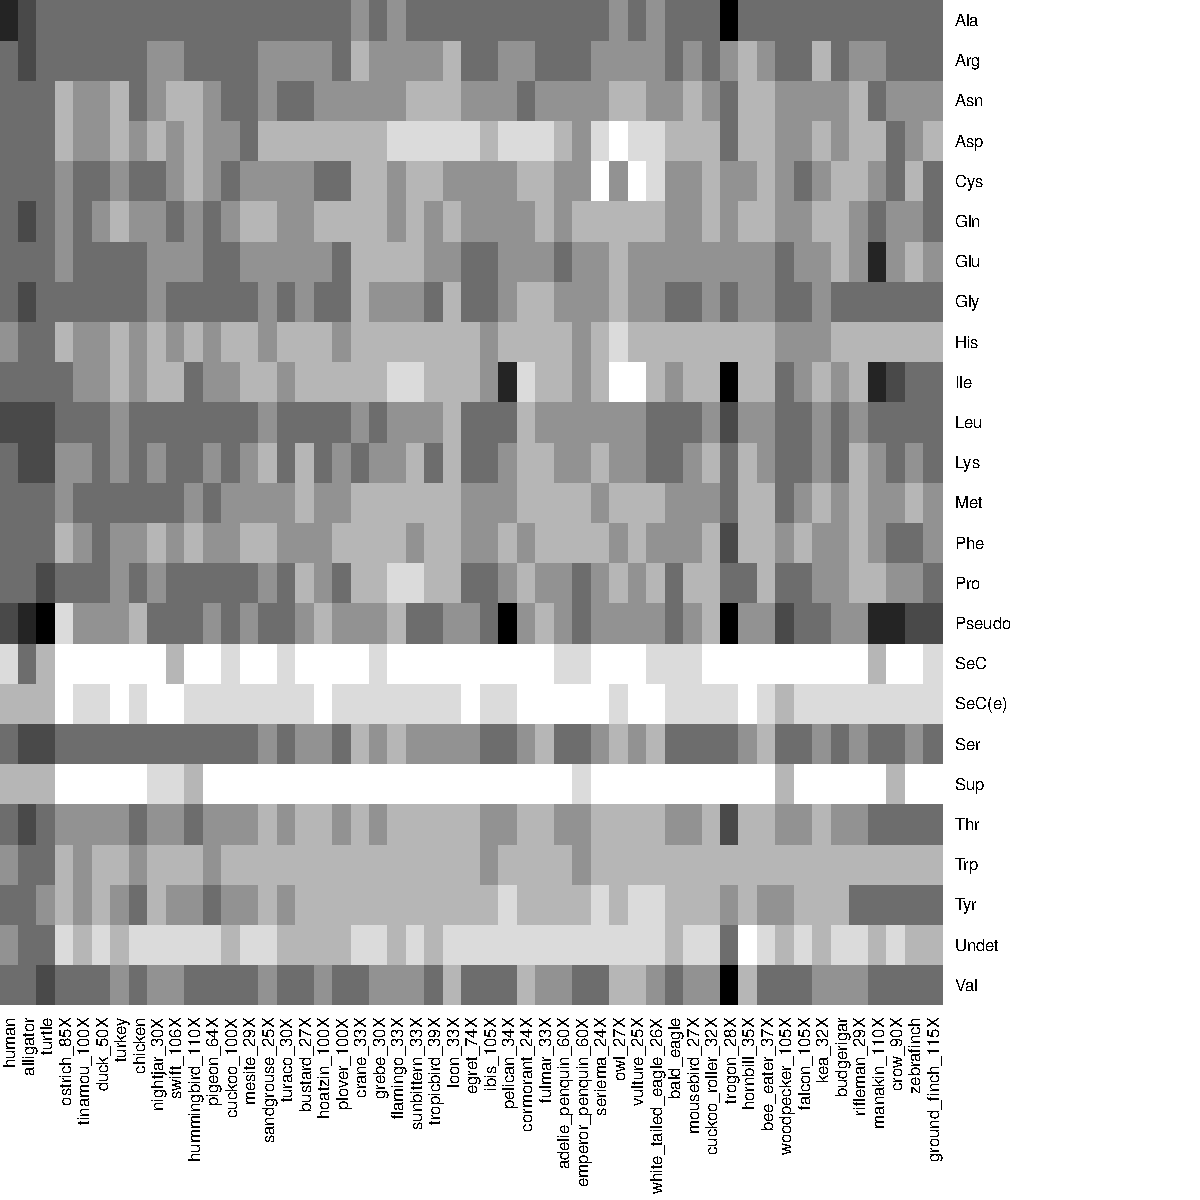
\includegraphics[width=0.45\textwidth]{figures/tRNA.pdf}
  \caption[]{Heatmaps showing the prescence/abscence and approximate
    copy number of {\bf lncRNA} families on the right and {\bf tRNA}
    families on the left.}\label{fig:5}
\end{figure}

\begin{figure}[ht]
  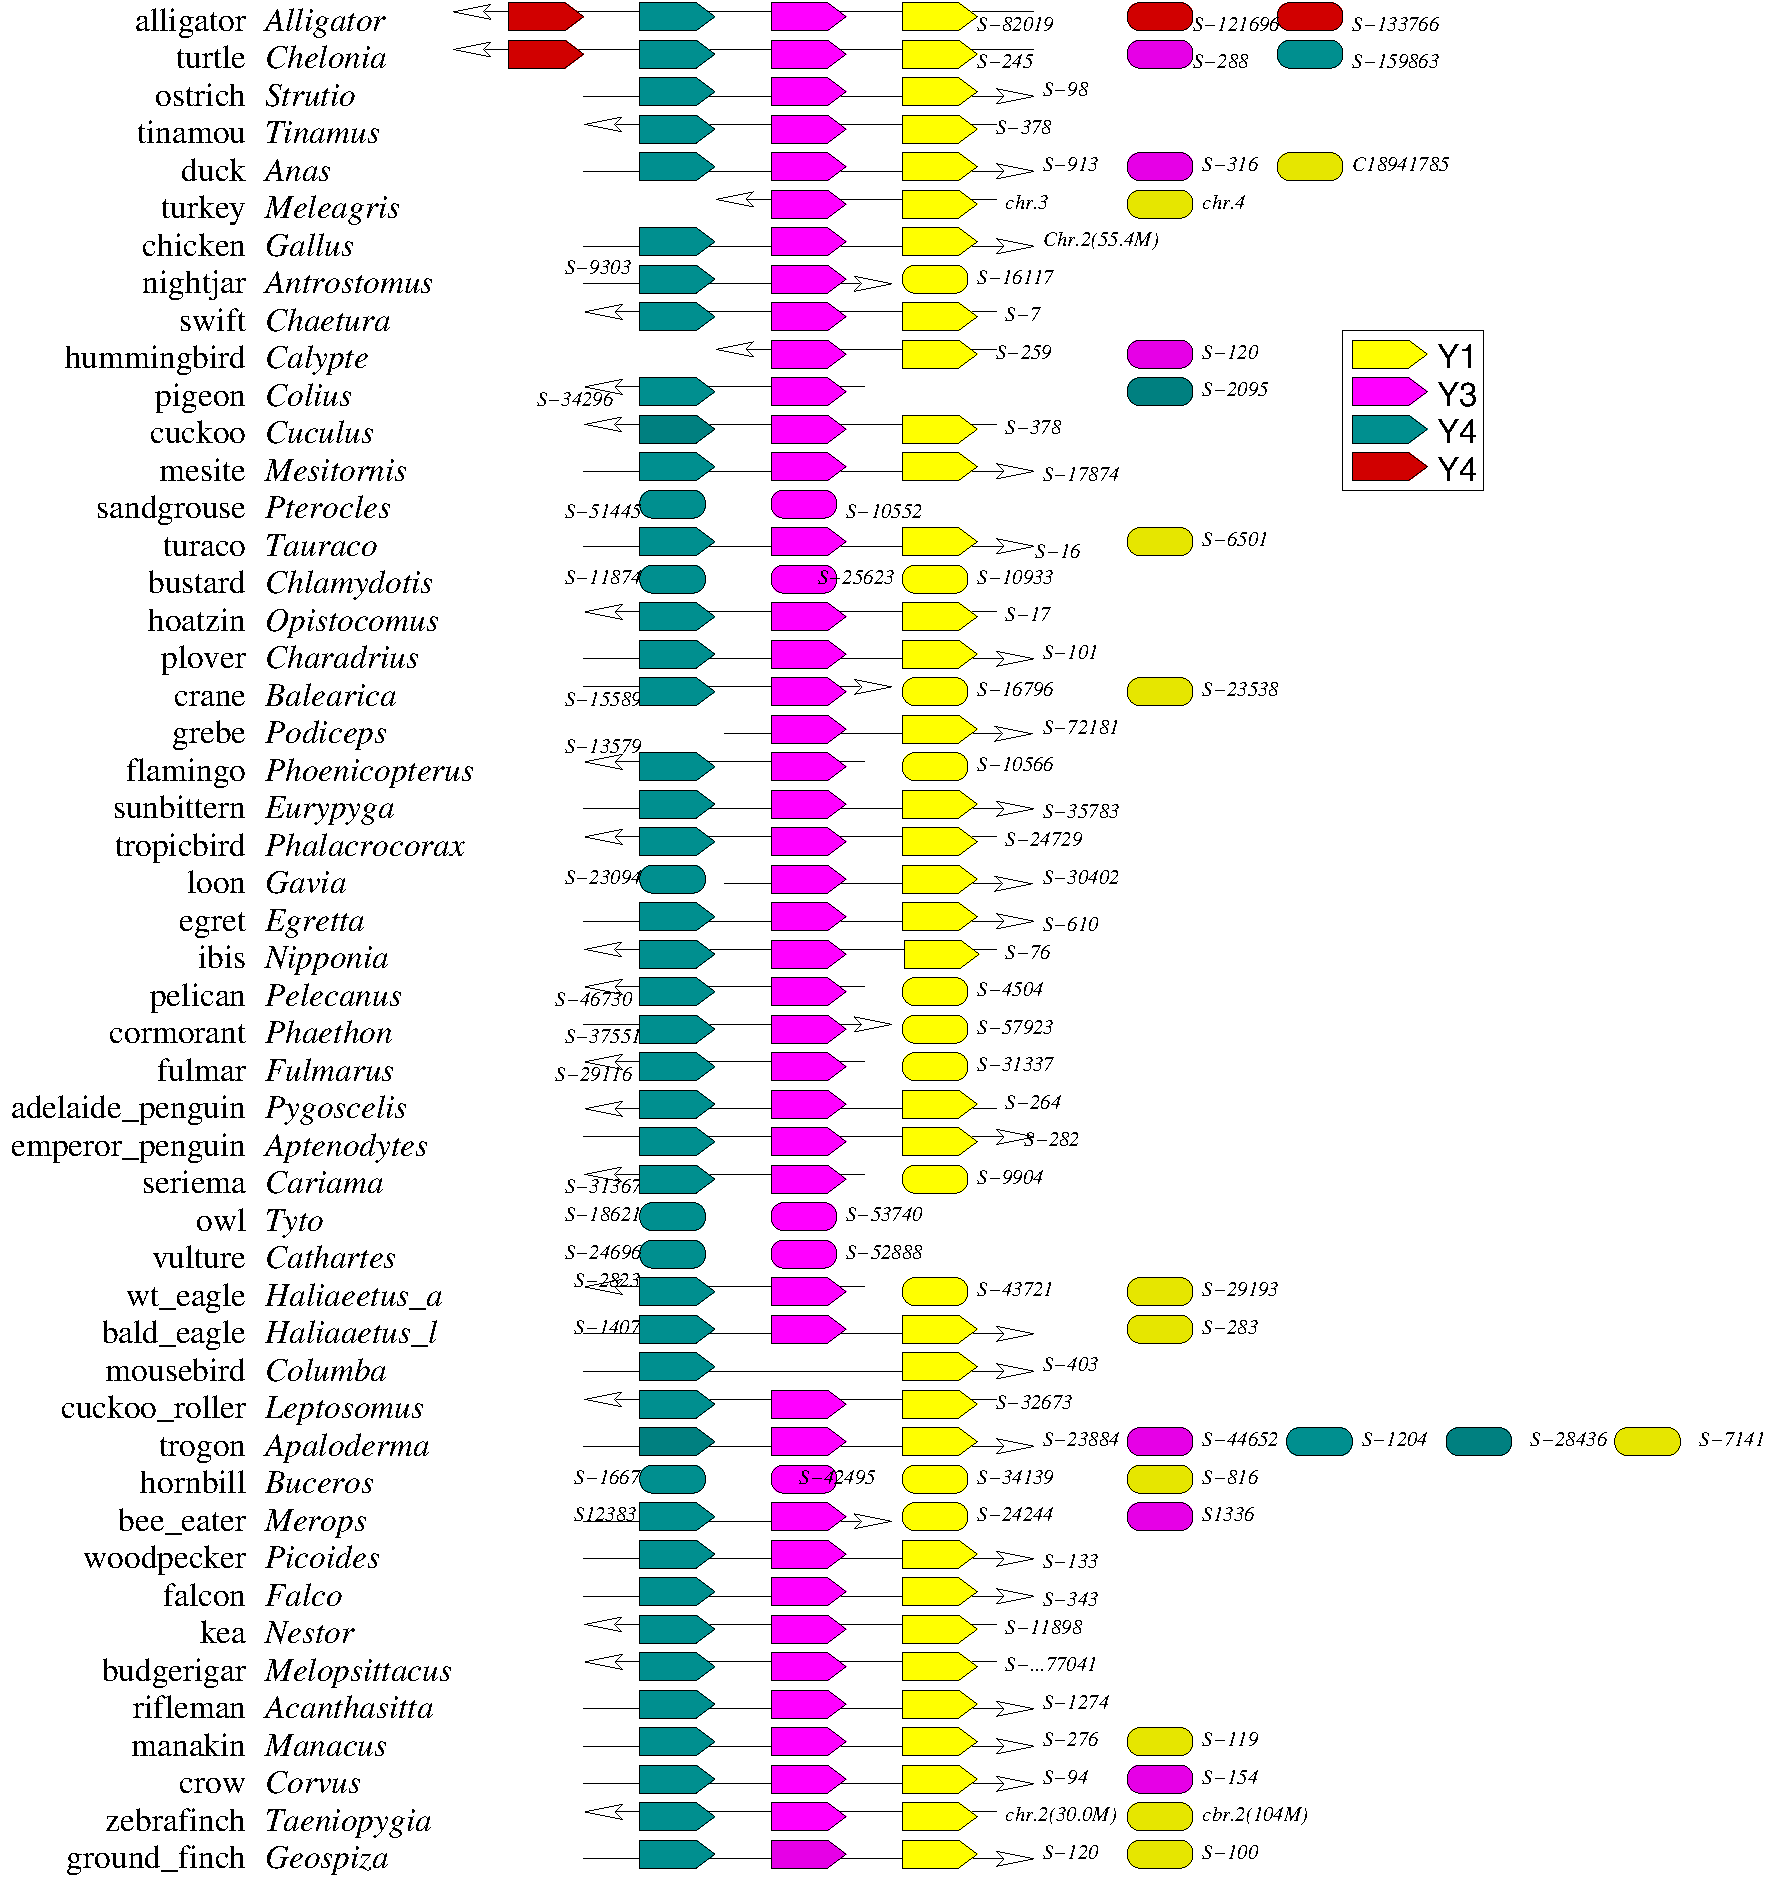
\includegraphics[width=0.45\textwidth]{figures/Y.pdf}
  \caption[]{...}\label{fig:6}
\end{figure}

\begin{figure}[ht]
  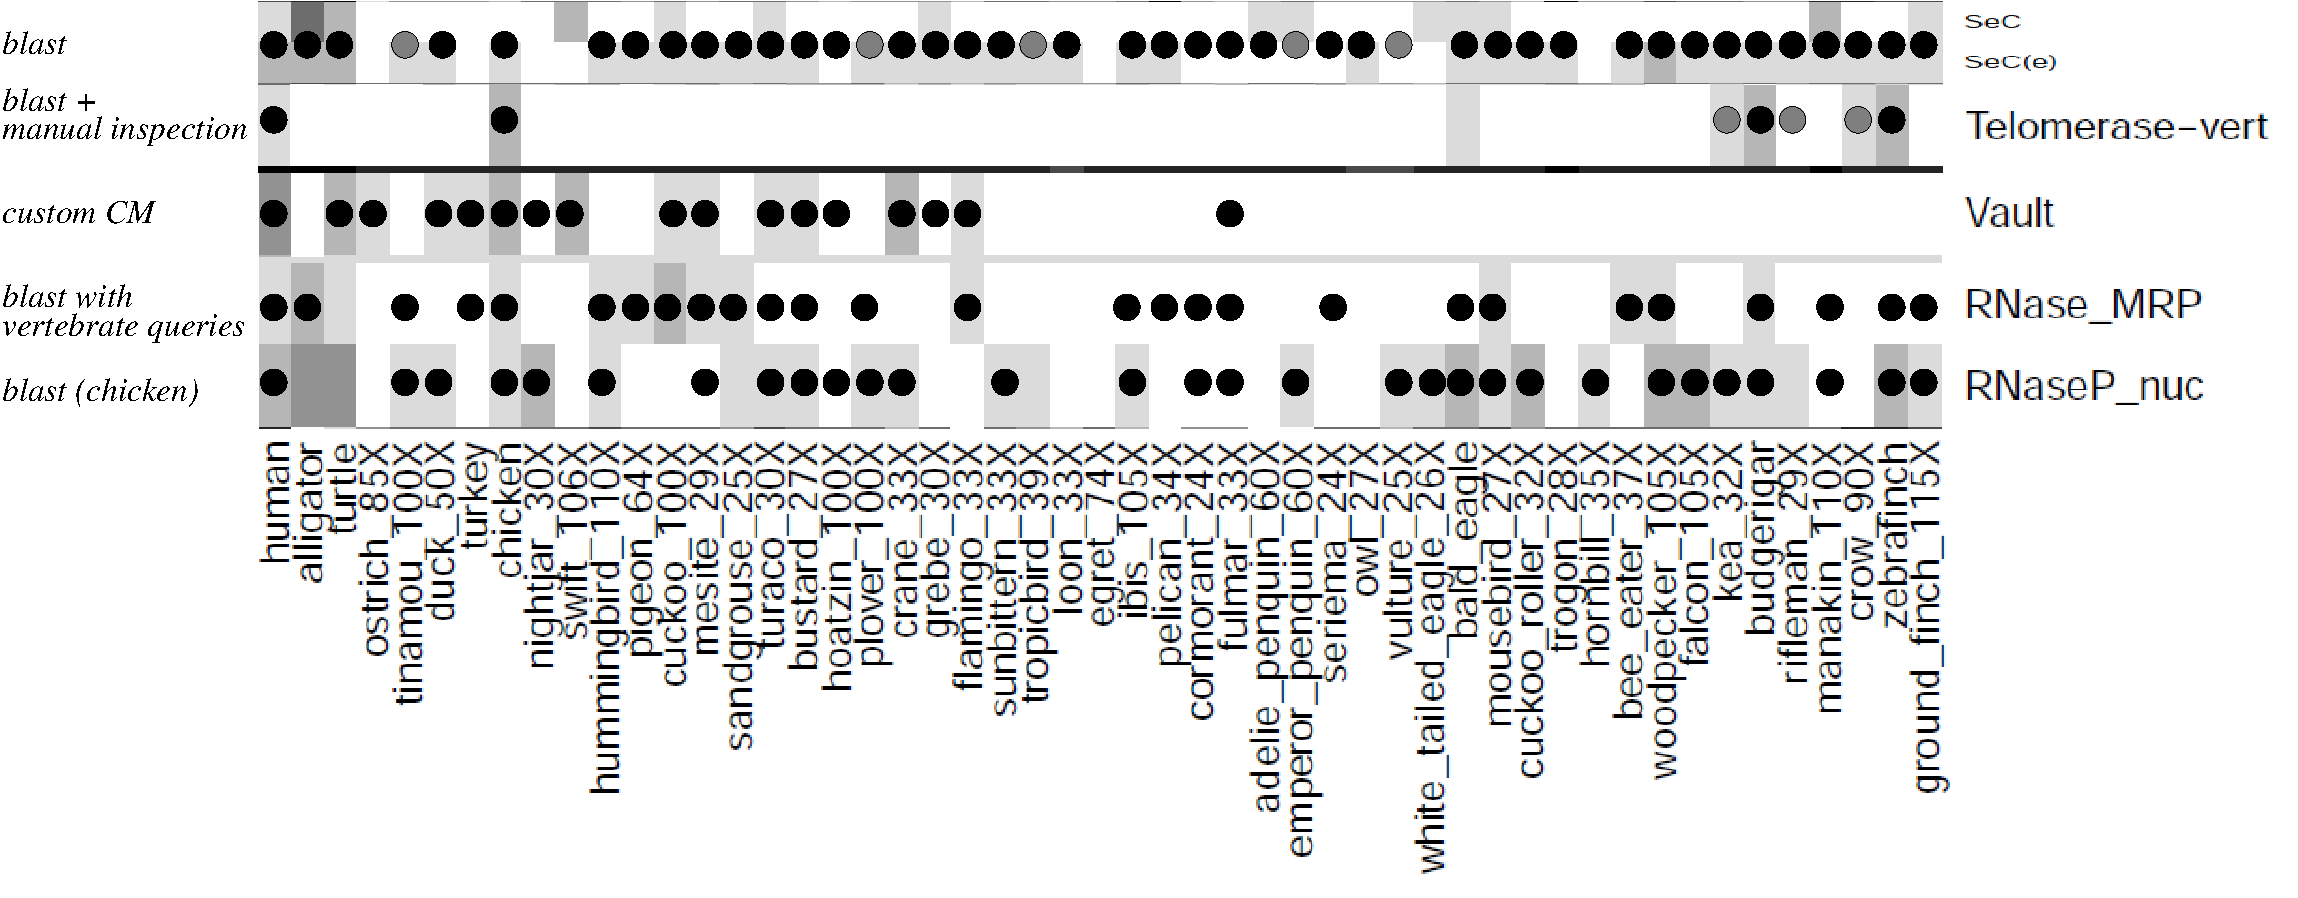
\includegraphics[width=0.45\textwidth]{figures/More-cand.pdf}
  \caption[]{...}\label{fig:7}
\end{figure}

\begin{figure}[ht]
  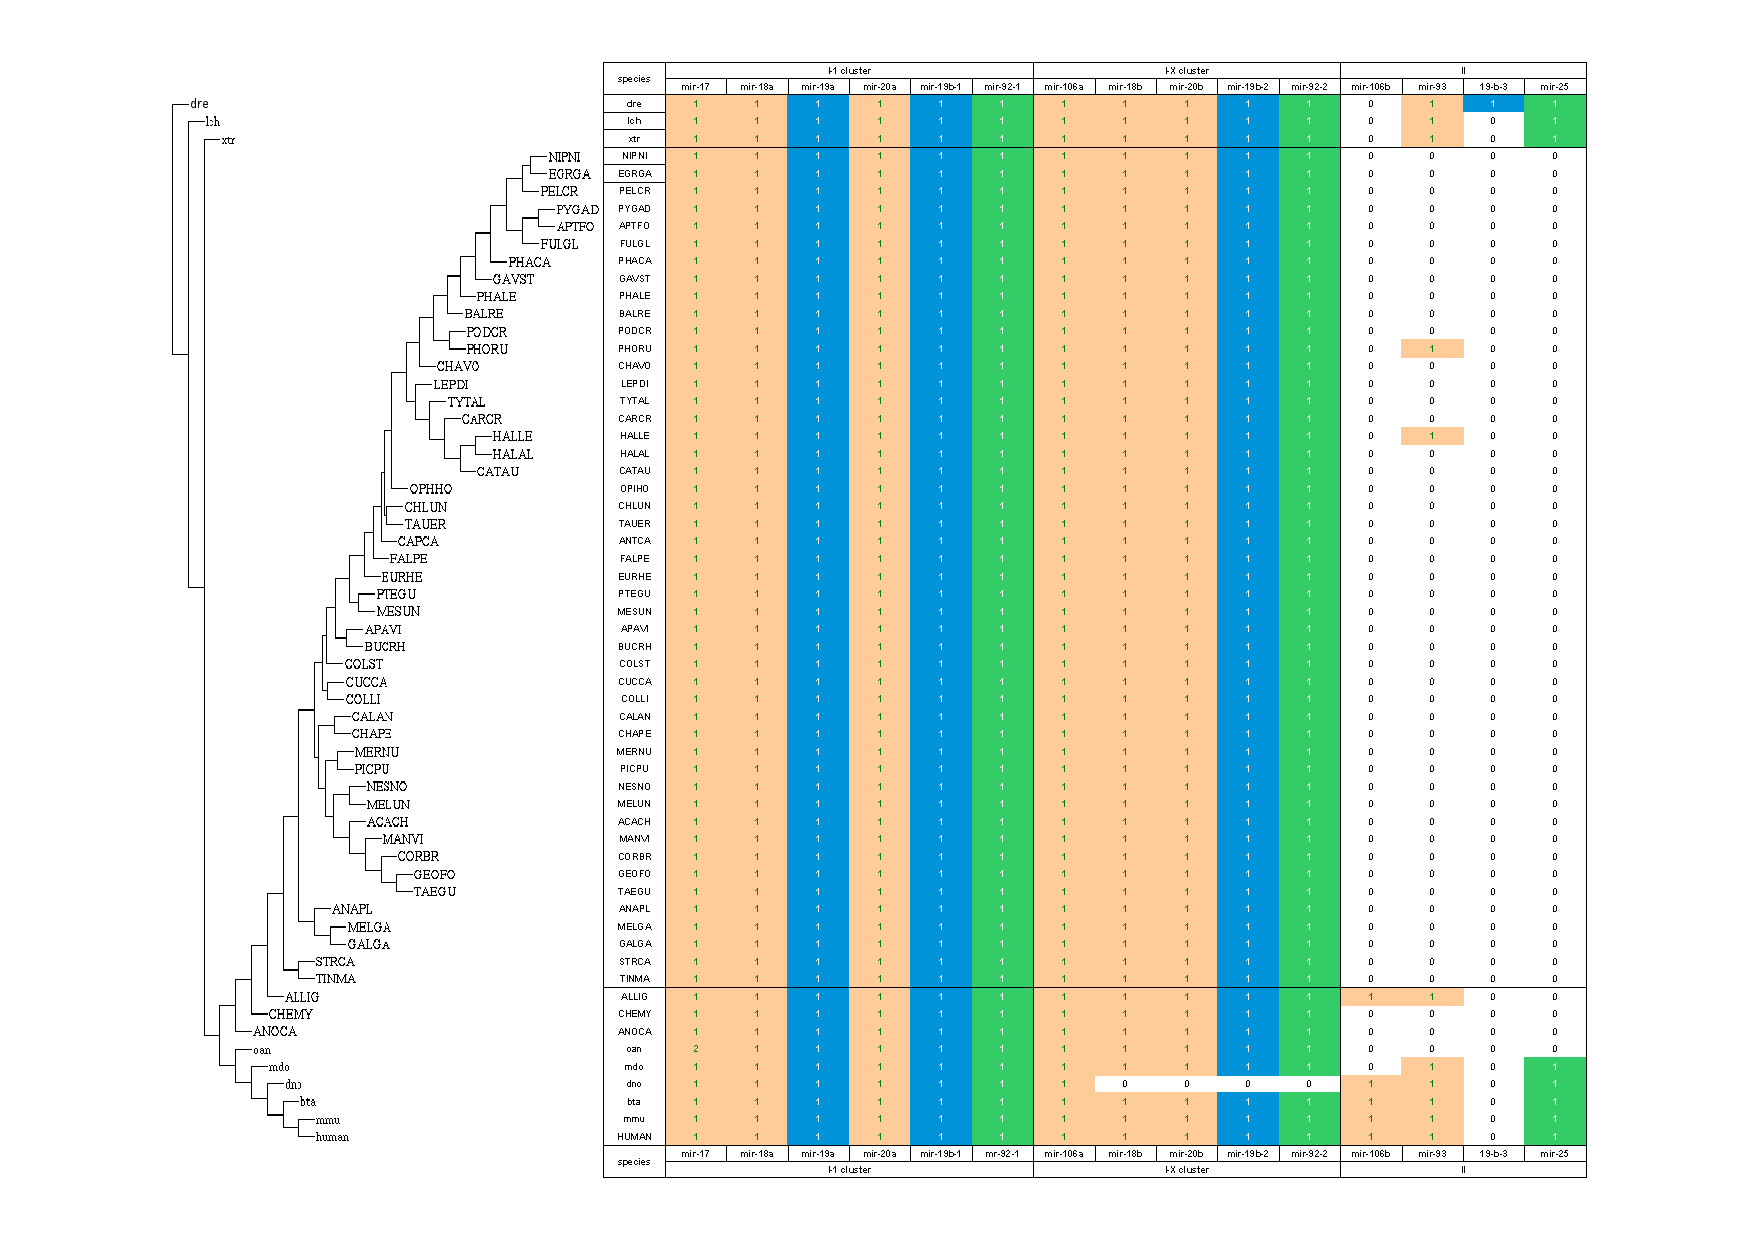
\includegraphics[width=0.45\textwidth]{figures/mir-17-cluster.pdf}
  \caption[]{...}\label{fig:8}
\end{figure}

\begin{figure}[ht]
  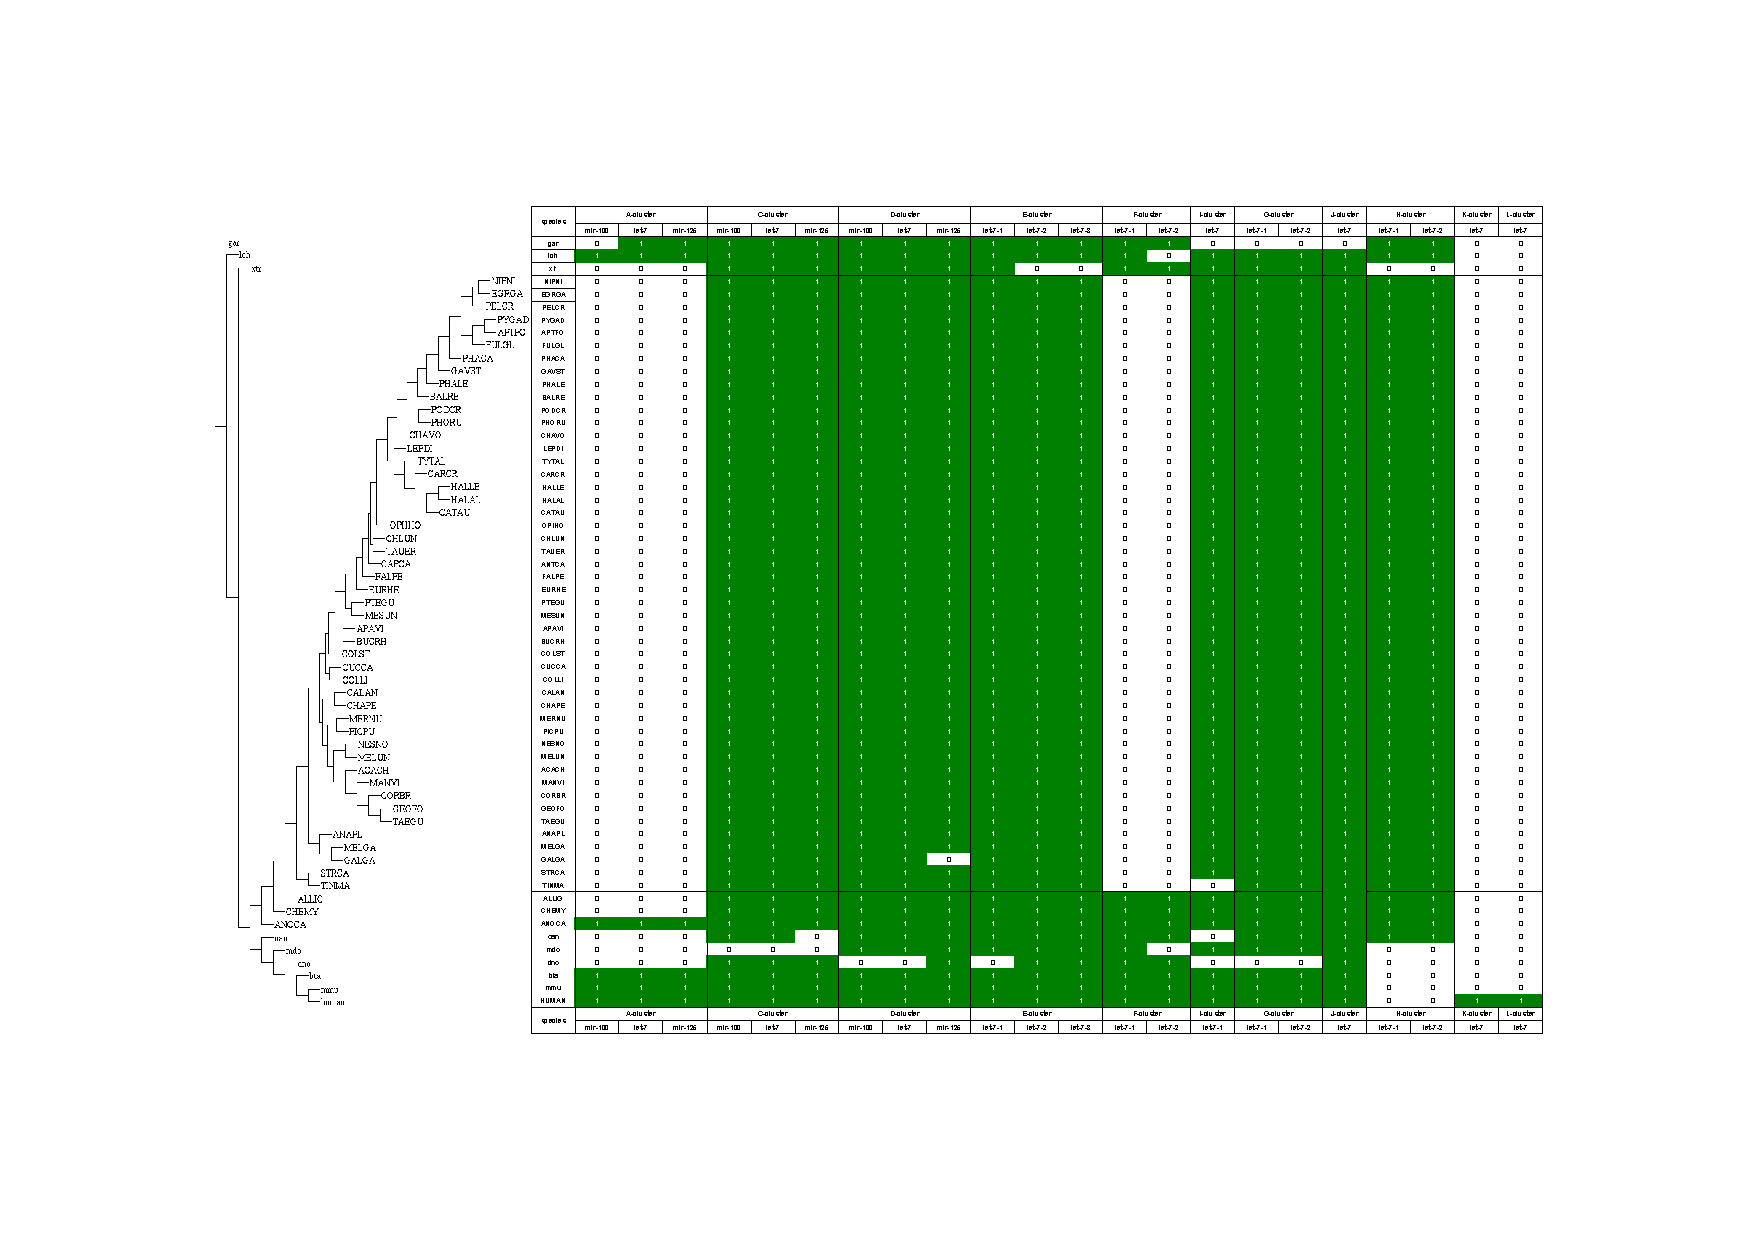
\includegraphics[width=0.45\textwidth]{figures/let-7-cluster.pdf}
  \caption[]{...}\label{fig:9}
\end{figure}



\end{bmcformat}
\end{document}

%%% Local Variables:
%%% mode: latex
%%% TeX-master: t
%%% End: 
